% Manuscript for Hydrology and Earth System Sciences (HESS).
% Portable article layout for review and the preprint; move into the Copernicus LaTeX template
% (copernicus.cls, https://publications.copernicus.org/for_authors/manuscript_preparation.html) at submission.
% Every number in the text comes from numbers.tex or tables/*.tex, generated by src/research/paper_figures.py.
\documentclass[11pt,a4paper]{article}
\usepackage[margin=25mm]{geometry}
\usepackage[T1]{fontenc}
\usepackage{lmodern}
\usepackage{microtype}
\usepackage{amsmath,amssymb}
\usepackage{graphicx}
\usepackage{booktabs}
\usepackage{adjustbox}
\usepackage[round,authoryear]{natbib}
\usepackage[hidelinks]{hyperref}
\usepackage{lineno}
\usepackage{textcomp}
\linenumbers
\graphicspath{{figures/}}
% Generated by src/research/paper_figures.py — do not edit by hand.
\newcommand{\nStations}{6,438}
\newcommand{\nManual}{5,516}
\newcommand{\nDWLR}{922}
\newcommand{\nObs}{414,106}
\newcommand{\nCampaigns}{246,887}
\newcommand{\nCampaignWells}{5,516}
\newcommand{\snapMedian}{3.6}
\newcommand{\imdMedian}{1,004}
\newcommand{\rechargeShare}{78}
\newcommand{\skillMzeroThree}{0.54}
\newcommand{\skillMzeroSix}{0.55}
\newcommand{\skillMzeroTwelve}{0.20}
\newcommand{\gainSixMSE}{5.0}
\newcommand{\gainSixMAE}{3.6}
\newcommand{\gainSixWins}{22}
\newcommand{\gainSixCampaigns}{24}
\newcommand{\oracleMin}{5.5}
\newcommand{\oracleMax}{9.6}
\newcommand{\oracleRobustMin}{2.5}
\newcommand{\splitShallow}{88}
\newcommand{\splitDeep}{46}
\newcommand{\aciWorstThree}{1.6}
\newcommand{\aciWorstSix}{1.7}
\newcommand{\aciWorstTwelve}{3.02}
\newcommand{\vmaxEoneThree}{0.43}
\newcommand{\vmaxEthreeSix}{0.69}
\newcommand{\valEoneThreeTrig}{0.37}
\newcommand{\hitEoneThree}{58}
\newcommand{\farEoneThree}{46}
\newcommand{\hitEthreeSix}{76}
\newcommand{\farEthreeSix}{48}
\newcommand{\valEthreeSixTrig}{0.58}


\title{Monsoon forcing, depth-aware calibration and decision value in national-scale groundwater forecasting for India}
\author{Akhil Golepu\thanks{Affiliation and ORCID to be completed by the author. Correspondence: akhilgolepu9@gmail.com}}
\date{Draft, October 2026}

\begin{document}
\maketitle

\begin{abstract}
Machine-learning forecasts of groundwater levels are increasingly proposed for water management in India, but three
questions that decide their usefulness remain open: whether monsoon rainfall adds skill beyond the memory of the aquifer,
whether forecast uncertainty can be trusted for shallow and deep wells alike, and whether the forecasts are worth acting on.
We address all three with \nObs{} quality-controlled readings from \nStations{} Central Ground Water Board monitoring wells
(1994--2025), a time-blocked design (train $\le$ 2015, calibrate 2016--2018, test 2019--2025) and nested gradient-boosting
models fed with gridded IMD rainfall and temperature and ENSO and Indian Ocean Dipole indices. A memory-only global model
removes \skillMzeroThree{}, \skillMzeroSix{} and \skillMzeroTwelve{} of the squared error of persistence at 3, 6 and 12
months. Observed monsoon forcing adds a small but robust gain, largest at 6 months (\gainSixMSE\,\% lower squared error, better
in \gainSixWins{} of \gainSixCampaigns{} test campaigns), that holds under an alternative split and in unseen regions; a
perfect rainfall forecast would add a further \oracleMin--\oracleMax\,\%. The single-day rainfall field distributed with
the widely used public compilation of these data carries no information (median 3.6\,mm per year), which explains an earlier
null result. A single conformal interval covers \splitShallow\,\% of readings in wells shallower than 5\,m but only
\splitDeep\,\% in wells deeper than 40\,m; intervals pooled by depth and region and updated online with adaptive conformal
inference keep every depth and region class within \aciWorstThree{}, \aciWorstSix{} and \aciWorstTwelve{} percentage points
of the nominal 80 and 90\,\% levels. Static calibration drifted because the wet 2019--2022 monsoons followed a dry
calibration period. Exceedance warnings carry substantial economic value once their probabilities are recalibrated on a
rolling window (peak relative value \vmaxEoneThree{} for deeper-than-usual levels at 3 months and \vmaxEthreeSix{} for
crossing an 8\,m pump-suction limit at 6 months), whereas raw probabilities lose value for most users. We recommend issuing
warnings when the forecast probability exceeds the user's cost--loss ratio and release the code, forecasts and an interactive
dashboard.
\end{abstract}

\section{Introduction}

India withdraws more groundwater than any other country, and the decline of its water tables under irrigated agriculture
has been documented from wells and from satellite gravimetry alike \citep{rodell2009india,asoka2017monsoon}. Most of the
country's aquifers are recharged during a single monsoon season, so the question a farmer, a district planner or a scheme
such as the Atal Bhujal Yojana asks before the dry season is concrete: how deep will the water be after the next monsoon,
how sure can we be, and is it worth acting on a warning?

Machine-learning models of groundwater levels have multiplied: a recent review synthesises 223 studies and finds feature
selection and tuning underdeveloped \citep{jesse2025review}, and many studies use a few dozen wells, random or single
splits and no naive baseline. At national scale,
\citet{malakar2021india} trained recurrent networks on more than 5\,000 Indian wells, and a 2026 open benchmark compared
tree ensembles, recurrent networks and the Chronos foundation model on the public compilation of Central Ground Water Board
(CGWB) levels used here \citep{alphoenixx2026benchmark}. Work on German networks has shown how global models with static
site descriptors behave \citep{heudorfer2024global,gomez2024cnn,ohmer2026gems}, and a recent study of Korean wells found
that known future weather, not site-specific learning, is the main source of short-horizon skill \citep{kim2026sources}.

Three gaps remain. First, it is not established how much monsoon forcing adds to groundwater memory at seasonal lead times
across India; the national benchmark found that climate features added almost nothing, but we show that the rainfall field
it relied on is a single-day snapshot. Second, interval forecasts are rarely checked for coverage conditional on aquifer
depth, region or season, and none of the studies we found used distribution-free (conformal) intervals for groundwater
levels. Third, no groundwater forecasting study we found has measured the decision value of its warnings, although the
cost--loss framework has been standard in weather forecasting for decades \citep{richardson2000value}.

We therefore ask: (RQ1) How much skill does monsoon forcing add to groundwater memory, and at which horizons, depths,
regions and seasons? (RQ2) Can prediction intervals hold their stated coverage for every depth and region class, and keep
holding when the climate regime shifts? (RQ3) Are exceedance warnings worth acting on, for whom and at what trigger?

\section{Data}

\subsection{Groundwater levels}
We use the public compilation of CGWB groundwater levels \citep{alphoenixx2026benchmark} (Table~\ref{tab:data}). The file
mixes two networks: manual wells read in four campaigns a year (January, May, August and November) and Digital Water Level
Recorder (DWLR) telemetry wells read several times a day since about 2023. The two use opposite sign conventions, which we
harmonise to depth below ground level by each station's majority sign. Physically impossible values ($<-5$\,m or
$>250$\,m) and per-station outliers (robust $z>8$) are removed. Manual readings are mapped to the nearest campaign, giving
\nCampaigns{} campaign values at \nCampaignWells{} wells (Fig.~\ref{fig:area}). Forecasts are made for these manual wells;
DWLR wells are used only for description.

\begin{table*}[t]
\caption{Data used in this study.}
\label{tab:data}
\centering\small
\begin{adjustbox}{max width=\textwidth}
\begin{tabular}{ll}
\toprule
Item & Value \\
\midrule
Stations (manual / DWLR) & 6,438 (5,516 / 922) \\
Readings after quality control & 414,106 \\
Period & 1994--2025 \\
Manual-well campaign values (Jan, May, Aug, Nov) & 246,887 from 5,516 wells \\
Split by target year & train $\le$ 2015; calibration 2016--2018; test 2019--2025 \\
Rainfall forcing & IMD 0.25$^\circ$ daily gridded, 1990--2025 \\
Temperature forcing & IMD 1$^\circ$ daily Tmax/Tmin, 1990--2025 \\
Teleconnections & Ni\~no 3.4 and DMI (HadISST, NOAA PSL), lags 0/3/6 months \\
\bottomrule
\end{tabular}
\end{adjustbox}
\end{table*}


\begin{figure*}[t]
\centering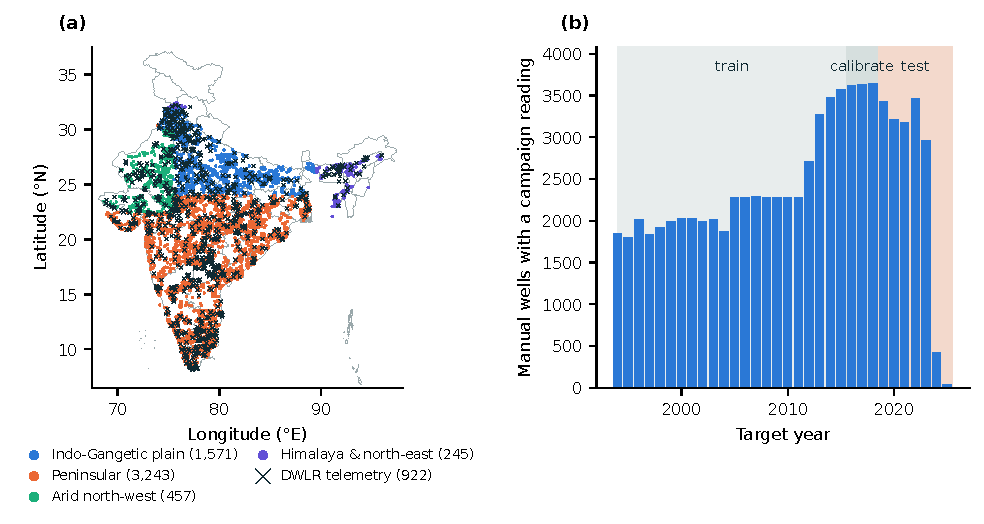
\includegraphics[width=\textwidth]{fig1}
\caption{(a) Monitoring wells by region (manual network) and DWLR telemetry wells. (b) Manual wells with a campaign
reading per target year and the time-blocked split.}
\label{fig:area}
\end{figure*}

\subsection{Forcing}
Daily rainfall on the IMD 0.25$^\circ$ grid \citep{pai2014imd} and daily maximum and minimum temperature on the
1$^\circ$ grid \citep{srivastava2009temp} were aggregated to monthly values for 1990--2025. Each well takes the nearest
grid cell with data. In the rainfall grid, 362 cell-years recorded zero rain all year while their neighbours received
hundreds of millimetres; these were replaced by the neighbours' mean, and 477 cell-years in contiguous zero blocks were set
to missing. Monthly Ni\~no~3.4 and Dipole Mode Index (DMI) series from HadISST \citep{rayner2003hadisst,saji1999dipole}
represent ENSO and the Indian Ocean Dipole.

Three checks support the forcing (Fig.~\ref{fig:forcing}). All-India June--September departures from our grid agree in sign
with IMD's published departures in all ten years checked. The May-to-November rise of the water table increases with the
season's rainfall at the well, positively at \rechargeShare\,\% of wells. And the rainfall column distributed with the
groundwater file is unrelated to real rainfall: summed over four campaigns it has a median of \snapMedian\,mm, against
\imdMedian\,mm of IMD rain over the previous year. That column holds rainfall on the day of the reading.

\begin{figure*}[t]
\centering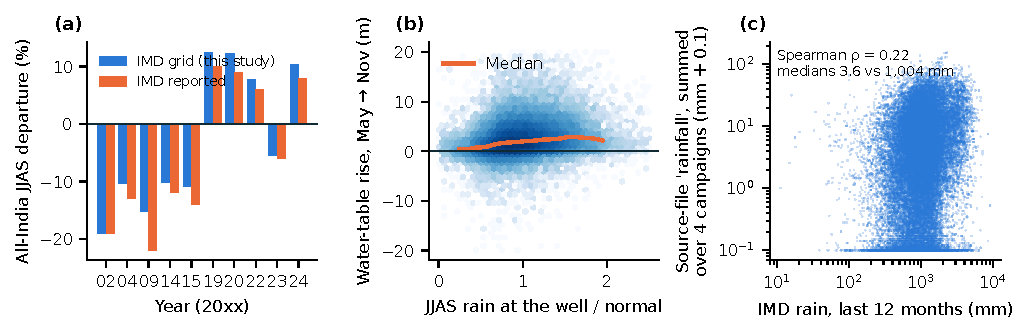
\includegraphics[width=\textwidth]{fig2}
\caption{Forcing checks. (a) All-India JJAS rainfall departures from the IMD grid and as reported by IMD. (b) Monsoon
recharge (May to November rise) against the season's rainfall relative to normal; line: binned median. (c) The rainfall
column of the source file against IMD rainfall over the previous 12 months.}
\label{fig:forcing}
\end{figure*}

\section{Methods}

\subsection{Forecasting task and validation design}
For each well and origin campaign $t$ we forecast the depth at $t+h$ for $h=1$, 2 and 4 campaigns (about 3, 6 and 12 months).
Rows are assigned by the year of the target: training $\le 2015$, calibration 2016--2018 and test 2019--2025, the same
boundary for every well. Features available at the origin are the current depth, four lags, changes over one and four
campaigns, origin and target season, an expanding per-well seasonal climatology (no look-ahead), the current anomaly,
record length, location and borehole depth. Forcing features use only months before the origin campaign month; climatologies
and SPI parameters \citep{mckee1993spi} are fitted on years up to 2015. Unit tests check that none of these features can see
data after the origin.

\subsection{Nested models (RQ1)}
All models are global XGBoost regressors \citep{chen2016xgboost} that predict the change $y_{t+h}-y_t$. Five arms are trained
on identical rows: \emph{M0} memory only; \emph{M1} adds past rainfall (since the previous campaign, 3, 6 and 12 months),
the last monsoon total and its ratio to normal, SPI-3/6/12 and the temperature anomaly; \emph{M2} adds Ni\~no~3.4 and DMI at
lags of 0, 3 and 6 months; \emph{M3} adds the rainfall that actually fell between origin and target, an oracle that bounds the
value of a perfect seasonal rainfall forecast; and the control \emph{C} adds the source file's single-day rainfall summed over
2, 4 and 8 campaigns, as in earlier work. Each arm receives the same search over six settings, early-stopped on target years
2013--2015 and refitted on all training years. We compare against persistence, seasonal naive, per-well climatology, anomaly
persistence, Random Forest and zero-shot Chronos-2 \citep{ansari2024chronos}.

Skill is the reduction in mean squared error relative to persistence. Confidence intervals come from a well-clustered
bootstrap (1\,000 draws). About 0.1\,\% of test readings are single-reading jumps of tens of metres, probably datum changes
or replaced wells, which carry about 15\,\% of the squared error. They remain in every headline number, but they make
squared-error Diebold--Mariano tests \citep{diebold1995comparing} uninformative, so we report the mean-absolute-error reduction
with clustered intervals and a two-sided sign test on the number of test campaigns in which the richer arm has the lower
error. Robustness is checked with an alternative split (train $\le$ 2017, test 2020--2025) and with five-fold cross-validation
over $2^\circ \times 2^\circ$ spatial blocks, which forecasts regions the model has not seen.

\subsection{Interval calibration (RQ2)}
Intervals wrap the M2 point forecast. Split conformal intervals \citep{lei2018distribution} use one pool of signed calibration
residuals with finite-sample ranks; Mondrian variants keep separate pools for depth class $\times$ season or depth class
$\times$ region, with fallback to the parent pool below 50 residuals; we also test Gaussian intervals, residuals normalised by
a cross-fitted spread model, and conformalised quantile regression \citep{romano2019cqr}. The online variant grows each pool
with test residuals whose target lies at least $h$ campaigns before the forecast's target (that is, already observed when the
forecast was issued) and adapts each cell's working $\alpha$ with adaptive conformal inference \citep{gibbs2021aci}, using a
step size $\gamma=0.05$ fixed before testing. Coverage is evaluated at 50, 80, 90 and 95\,\% overall and by depth, region,
season and record length, with binomial tests and Holm correction, the Winkler score and CRPS \citep{gneiting2007scoring}.
Our acceptance criterion is that every depth and region class stays within 3 points of nominal at 80 and 90\,\%.

\subsection{Warnings and decision value (RQ3)}
We define three events at the target: E1, depth deeper than the well's own 80th percentile for that season; E2, a standardised
groundwater index below $-1$ \citep{bloomfield2013sgi}; and E3, for wells currently at 8\,m or shallower, the water falling
below 8\,m, where centrifugal surface pumps lose suction. Thresholds use readings up to 2018. The raw probability of an event
is the share of residuals in the online depth $\times$ region pool that would place the forecast beyond the threshold. Because
interval calibration does not imply calibration at every threshold, we also recalibrate probabilities with isotonic regression
\citep{zadrozny2002isotonic}, either once on 2016--2018 or on a rolling window of the eight most recent campaigns whose outcomes
were known at issue time. Probabilities are scored with the Brier skill score \citep{brier1950verification} against each well's
own climatological frequency and with ROC AUC. Decision value is the relative economic value $V$ of \citet{richardson2000value}
for a user who pays $C$ to protect against a loss $L$ and acts when $p \ge C/L$; $V=1$ is a perfect forecast and $V=0$ is no
better than always or never acting. Intervals come from a paired well-clustered bootstrap.

\section{Results}

\subsection{How much does monsoon forcing add? (RQ1)}

Groundwater memory carries most of the skill (Table~\ref{tab:skill}, Fig.~\ref{fig:skill}). The memory-only model removes
\skillMzeroThree, \skillMzeroSix{} and \skillMzeroTwelve{} of persistence's squared error at 3, 6 and 12 months, well ahead of
anomaly persistence. Adding observed forcing and ENSO/IOD (M2) improves on memory alone in every horizon and setting
(Table~\ref{tab:gains}): by 1.1, \gainSixMSE{} and 1.3\,\% of squared error and by 2.0, \gainSixMAE{} and 1.5\,\% of absolute error,
with absolute-error intervals that exclude zero at all horizons. The gain is clearest at 6 months, where the forcing arm is
better in \gainSixWins{} of \gainSixCampaigns{} test campaigns ($p<0.001$) and remains positive under the alternative split
(3.1\,\%) and in unseen regions (3.7\,\%). Rainfall alone (M1) adds less and loses its 12-month gain in unseen regions.

The gain is physically placed (Fig.~\ref{fig:strata}). It concentrates in the forecast that spans the monsoon, May to
November, where M2 cuts squared error by 12\,\% at 6 months, and in wells shallower than 15\,m. Deep wells and the
Himalaya and north-east gain little. Knowing the rain that actually fell (M3) would add a further \oracleMin--\oracleMax\,\% in
the main split (at least \oracleRobustMin\,\% in every robustness setting), growing with horizon; this is the skill a seasonal
monsoon forecast could unlock. The single-day rainfall of the source file adds nothing (C vs M0: $-2.1$ to $+0.2$\,\%),
which reproduces the earlier null result and shows that it came from the feature, not the hydrology. Chronos-2 used zero-shot
trails the trained models (skill 0.40 at 3 months against 0.51 for XGBoost on the same rows), although rainfall covariates
reduce its absolute error by 6--7\,\% at 3 and 6 months, and Random Forest performs like XGBoost.

\begin{table*}[t]
\caption{Test-period (2019--2025) point skill on identical rows: RMSE (m) and MSE skill against persistence with 95\,\% well-clustered bootstrap intervals.}
\label{tab:skill}
\centering\small
\begin{adjustbox}{max width=\textwidth}
\begin{tabular}{lrrrrrr}
\toprule
Model & RMSE 3 mo & Skill 3 mo & RMSE 6 mo & Skill 6 mo & RMSE 12 mo & Skill 12 mo \\
\midrule
Persistence & 3.48 & 0 & 4.17 & 0 & 3.17 & 0 \\
Anomaly persistence & 2.69 & 0.404 [0.354, 0.446] & 3.11 & 0.444 [0.393, 0.484] & 3.17 & 0.000 [0.000, 0.000] \\
C: snapshot rainfall & 2.38 & 0.531 [0.496, 0.561] & 2.80 & 0.550 [0.512, 0.584] & 2.87 & 0.185 [0.143, 0.226] \\
M0: memory & 2.37 & 0.536 [0.503, 0.563] & 2.80 & 0.549 [0.506, 0.586] & 2.84 & 0.201 [0.166, 0.235] \\
M1: + past forcing & 2.36 & 0.539 [0.503, 0.568] & 2.75 & 0.564 [0.526, 0.598] & 2.82 & 0.212 [0.179, 0.244] \\
M2: + ENSO/IOD & 2.36 & 0.541 [0.507, 0.569] & 2.73 & 0.572 [0.529, 0.608] & 2.82 & 0.212 [0.179, 0.243] \\
M3: + oracle rain & 2.29 & 0.566 [0.536, 0.592] & 2.65 & 0.598 [0.559, 0.633] & 2.68 & 0.287 [0.256, 0.316] \\
\bottomrule
\end{tabular}
\end{adjustbox}
\par\smallskip\begin{minipage}{0.95\textwidth}\footnotesize Rows: 25,340 / 24,073 / 32,472 forecasts at 3 / 6 / 12 months.\end{minipage}
\end{table*}

\begin{table*}[t]
\caption{Skill added between nested arms. MSE and MAE reduction (\%, MAE with 95\,\% well-clustered interval), test campaigns in which the richer arm has lower MAE with a two-sided sign test, and MSE reduction under an alternative split and spatially blocked validation.}
\label{tab:gains}
\centering\small
\begin{adjustbox}{max width=\textwidth}
\begin{tabular}{llrrrrrr}
\toprule
Comparison & Horizon & MSE & MAE & Campaigns & Sign $p$ & Alt. split & Unseen regions \\
\midrule
M1 vs M0 & 3 months & +0.7 & +1.2 [+0.6, +1.8] & 13/24 & 0.839 & +2.8 & +0.2 \\
 & 6 months & +3.3 & +1.5 [+1.0, +2.0] & 19/24 & 0.007 & +1.8 & +2.2 \\
 & 12 months & +1.3 & +1.9 [+1.5, +2.2] & 22/25 & $<$0.001 & +2.7 & $-$1.4 \\
M2 vs M0 & 3 months & +1.1 & +2.0 [+1.4, +2.6] & 16/24 & 0.152 & +3.0 & +2.0 \\
 & 6 months & +5.0 & +3.6 [+3.1, +4.0] & 22/24 & $<$0.001 & +3.1 & +3.7 \\
 & 12 months & +1.3 & +1.5 [+1.1, +2.0] & 17/25 & 0.108 & +5.7 & +1.0 \\
M3 vs M2 & 3 months & +5.5 & +3.4 [+2.9, +3.9] & 19/24 & 0.007 & +2.8 & +2.5 \\
 & 6 months & +6.1 & +4.2 [+3.5, +4.8] & 15/24 & 0.307 & +5.2 & +5.9 \\
 & 12 months & +9.6 & +6.5 [+5.8, +7.1] & 20/25 & 0.004 & +9.3 & +5.5 \\
C vs M0 & 3 months & $-$1.0 & $-$0.5 [$-$0.9, $-$0.1] & 10/24 & 0.541 & -- & -- \\
 & 6 months & +0.2 & +0.5 [+0.0, +0.9] & 14/24 & 0.541 & -- & -- \\
 & 12 months & $-$2.1 & +0.1 [$-$0.2, +0.5] & 12/25 & 1.000 & -- & -- \\
\bottomrule
\end{tabular}
\end{adjustbox}
\end{table*}


\begin{figure*}[t]
\centering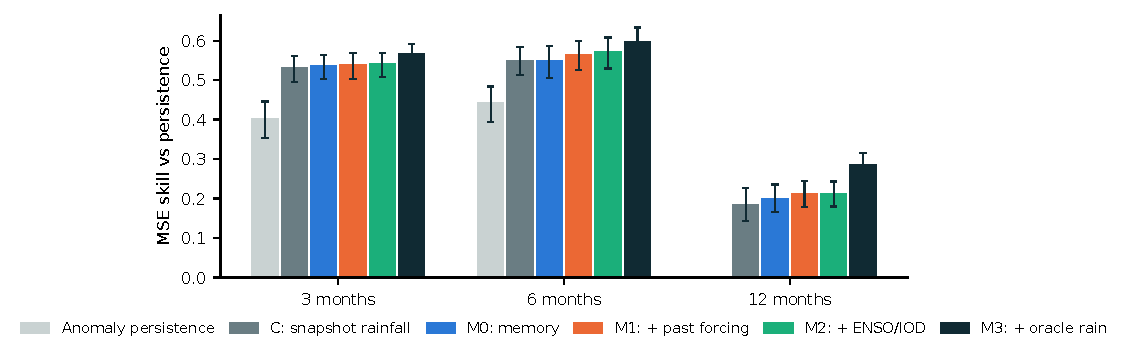
\includegraphics[width=\textwidth]{fig3}
\caption{Skill against persistence by arm and horizon on identical test rows; bars are 95\,\% well-clustered bootstrap
intervals.}
\label{fig:skill}
\end{figure*}

\begin{figure}[t]
\centering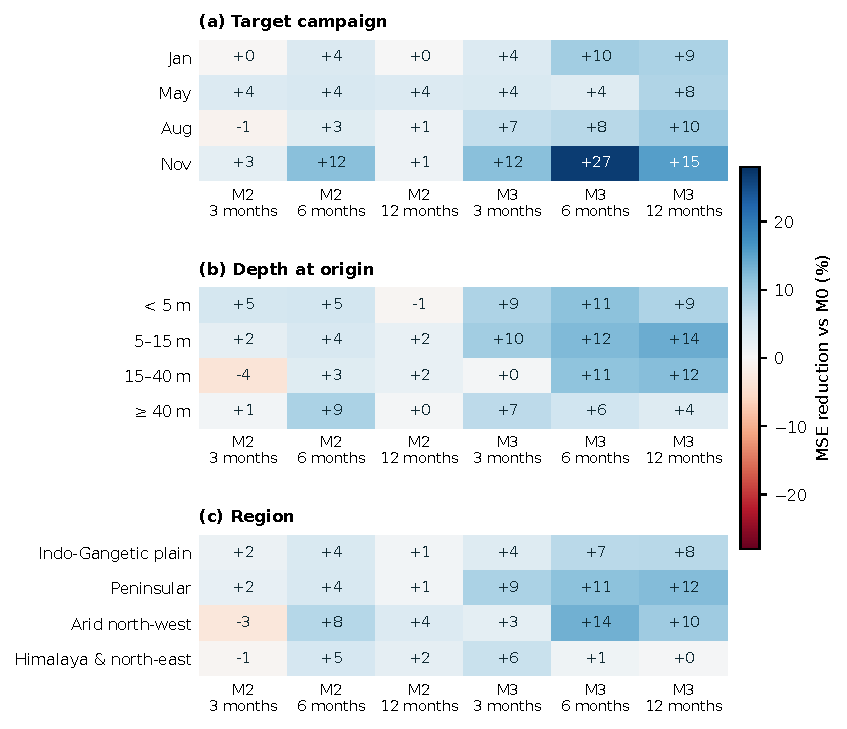
\includegraphics[width=0.85\textwidth]{fig4}
\caption{Reduction in squared error over the memory-only model by (a) target campaign, (b) depth at the origin and (c)
region, for M2 (observed forcing) and M3 (oracle rainfall).}
\label{fig:strata}
\end{figure}

\subsection{Can the intervals be trusted for every well? (RQ2)}

A single interval width fails by depth (Fig.~\ref{fig:coverage}, Table~\ref{tab:calib}): the 80\,\% split-conformal interval
covers \splitShallow\,\% of readings in wells shallower than 5\,m but \splitDeep\,\% in wells deeper than 40\,m, and Gaussian
intervals over-cover by ten points overall because the datum jumps inflate the residual spread, yet still fail by depth. Pools
by depth and region repair most of this, but static calibration under-covers by 2--5 points overall. The cause is a change of
regime (Fig.~\ref{fig:drift}): the calibration years 2016--2018 followed the 2014--2015 droughts, when water tables came in
deeper than forecast, while the strong 2019, 2020 and 2022 monsoons left water shallower than forecast, by a median of up to
0.68\,m at 12 months in 2022.

The online depth $\times$ region method with adaptive conformal inference absorbs the shift. It keeps every depth and region
class within \aciWorstThree, \aciWorstSix{} and \aciWorstTwelve{} points of nominal at 80 and 90\,\% at 3, 6 and 12 months. The
one cell beyond 3 points is the Himalaya and north-east at 12 months, which over-covers at 83.0\,\% with 854 readings (Holm-adjusted
$p=0.23$); we did not retune $\gamma$ on the test period to remove it. Two variants added after inspecting the results
(Table~\ref{tab:calib}, marked) also fix residual season misses and sharpen intervals, at the cost of slightly larger region
misses. Conformalised quantile regression and normalised conformal intervals are sharper but miss individual depth or region
classes by up to 9.4 points.

\begin{table*}[t]
\caption{Interval calibration in the test period: overall coverage of the 80\,\% interval (\%), the worst absolute deviation from nominal over depth and region classes at 80\,\% and 90\,\% (points), and the Winkler score (m).}
\label{tab:calib}
\centering\small
\begin{adjustbox}{max width=\textwidth}
\begin{tabular}{lrrrrrrrrr}
\toprule
Method & Cov. & Worst & Winkler & Cov. & Worst & Winkler & Cov. & Worst & Winkler \\
\midrule
Gaussian & 90.0 & 26.2 & 9.20 & 89.5 & 19.3 & 10.23 & 89.2 & 21.4 & 10.22 \\
Split conformal & 80.2 & 33.6 & 8.62 & 78.3 & 28.6 & 9.79 & 77.5 & 30.9 & 10.00 \\
Mondrian D$\times$S & 78.0 & 10.9 & 8.12 & 76.7 & 11.4 & 9.29 & 75.4 & 15.1 & 9.44 \\
Mondrian D$\times$R & 78.0 & 8.8 & 8.05 & 76.5 & 4.9 & 9.18 & 75.2 & 5.8 & 9.34 \\
Normalised & 78.0 & 6.2 & 7.29 & 77.2 & 7.1 & 8.24 & 76.6 & 8.8 & 8.25 \\
CQR & 80.5 & 4.4 & 7.03 & 79.5 & 6.2 & 7.99 & 80.3 & 9.4 & 8.02 \\
Mondrian D$\times$R + recal & 78.9 & 2.3 & 7.97 & 77.9 & 2.9 & 9.02 & 77.0 & 4.0 & 9.11 \\
Mondrian D$\times$R + recal + ACI & 79.3 & 1.6 & 7.99 & 79.9 & 1.7 & 9.04 & 78.7 & 3.0 & 9.12 \\
Mondrian D$\times$R$\times$S + recal + ACI$^\dagger$ & 78.6 & 2.6 & 8.00 & 77.9 & 2.9 & 9.08 & 77.5 & 3.6 & 9.05 \\
Normalised D$\times$R$\times$S + recal + ACI$^\dagger$ & 78.4 & 2.1 & 7.29 & 78.0 & 3.6 & 8.18 & 78.4 & 3.3 & 8.02 \\
\bottomrule
\end{tabular}
\end{adjustbox}
\par\smallskip\begin{minipage}{0.95\textwidth}\footnotesize Column groups: 3, 6 and 12 months. $^\dagger$ Added after inspecting results (post hoc).\end{minipage}
\end{table*}


\begin{figure*}[t]
\centering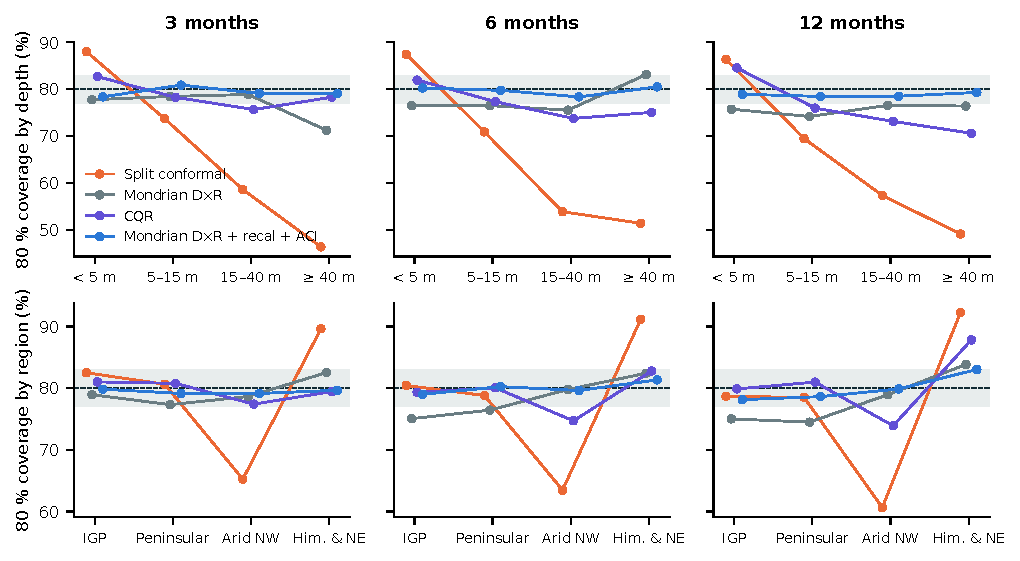
\includegraphics[width=\textwidth]{fig5}
\caption{Coverage of 80\,\% intervals by depth class (top) and region (bottom); the grey band marks $\pm3$ points around the
target.}
\label{fig:coverage}
\end{figure*}

\begin{figure}[t]
\centering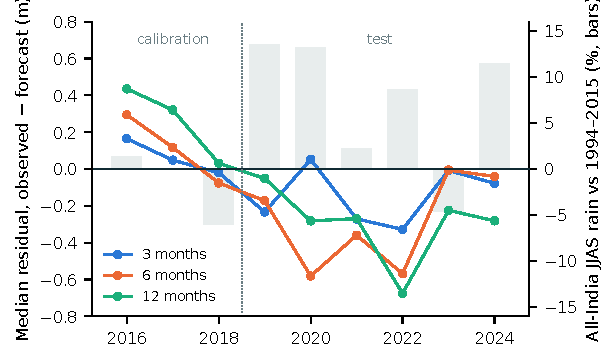
\includegraphics[width=0.75\textwidth]{fig6}
\caption{Median residual (observed minus forecast depth) of M2 by target year, with all-India JJAS rainfall anomaly
relative to 1994--2015 as bars.}
\label{fig:drift}
\end{figure}

\subsection{Are the warnings worth acting on? (RQ3)}

Raw warning probabilities are over-confident (Fig.~\ref{fig:reliability}): a predicted 55\,\% verified 33--41\,\% of the time.
Recalibration once on 2016--2018 over-corrects on the test years, the same drift as in RQ2, whereas the rolling recalibration
follows the diagonal and raises the Brier skill score at every horizon (Table~\ref{tab:value}). With rolling-recalibrated
probabilities, warnings carry positive value for nearly every cost--loss ratio (Fig.~\ref{fig:value}). Peak relative value is
\vmaxEoneThree{} for E1 at 3 months and \vmaxEthreeSix{} for E3 at 6 months. Observed forcing adds a small value gain at 6 months
only (+0.01 to +0.04 for $C/L$ between 0.1 and 0.5), and the oracle rainfall arm adds up to 0.13, again pointing to seasonal
rainfall forecasts as the next source of value.

At a trigger of 0.3, three-month E1 warnings are issued for about a quarter of forecasts, catch \hitEoneThree\,\% of events with
\farEoneThree\,\% of warnings not verifying, and give $V=\valEoneThreeTrig$. At a trigger of 0.2, six-month E3 warnings catch
\hitEthreeSix\,\% of crossings of the suction limit with \farEthreeSix\,\% of warnings not verifying ($V=\valEthreeSixTrig$). In the
dry 2023--2024 water year, exceedances in the Atal Bhujal states rose from 17\,\% to 25\,\% of readings while the mean warning
probability barely moved (0.16 to 0.17): the forecasts lagged the turn to a dry regime.

\begin{table*}[t]
\caption{Warning skill and value for model M2 with rolling-isotonic probabilities: event base rate, Brier skill score against each well's climatology (95\,\% interval), ROC AUC, peak relative economic value and the cost--loss ratio at which it occurs, and the range of cost--loss ratios with positive value.}
\label{tab:value}
\centering\small
\begin{adjustbox}{max width=\textwidth}
\begin{tabular}{llrrrrrr}
\toprule
Event & Horizon & Base rate & BSS & AUC & $V_{\max}$ & at $C/L$ & $V>0$ for $C/L$ \\
\midrule
Deeper than usual & 3 months & 0.24 & 0.234 [0.216, 0.250] & 0.79 & 0.43 & 0.24 & 0.02--0.96 \\
 & 6 months & 0.24 & 0.165 [0.149, 0.183] & 0.74 & 0.32 & 0.24 & 0.06--0.92 \\
 & 12 months & 0.25 & 0.143 [0.126, 0.159] & 0.71 & 0.27 & 0.24 & 0.06--0.98 \\
SGI $<-1$ & 3 months & 0.19 & 0.265 [0.239, 0.293] & 0.81 & 0.45 & 0.18 & 0.02--0.92 \\
 & 6 months & 0.19 & 0.207 [0.181, 0.233] & 0.78 & 0.38 & 0.18 & 0.04--0.90 \\
 & 12 months & 0.19 & 0.185 [0.158, 0.212] & 0.75 & 0.32 & 0.20 & 0.04--0.90 \\
Below 8 m & 3 months & 0.09 & 0.336 [0.306, 0.365] & 0.91 & 0.65 & 0.08 & 0.02--0.68 \\
 & 6 months & 0.10 & 0.255 [0.224, 0.287] & 0.92 & 0.69 & 0.10 & 0.02--0.74 \\
 & 12 months & 0.06 & 0.253 [0.220, 0.285] & 0.86 & 0.54 & 0.06 & 0.02--0.46 \\
\bottomrule
\end{tabular}
\end{adjustbox}
\end{table*}


\begin{figure*}[t]
\centering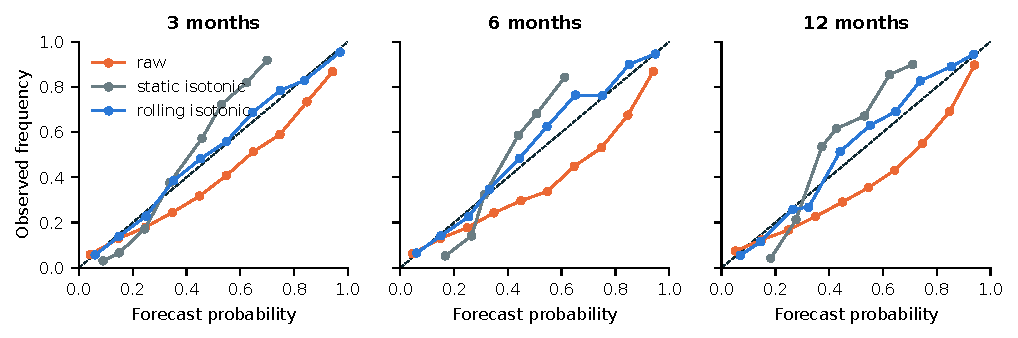
\includegraphics[width=\textwidth]{fig7}
\caption{Reliability of E1 warning probabilities from M2: raw, recalibrated once on 2016--2018, and recalibrated on a rolling
window.}
\label{fig:reliability}
\end{figure*}

\begin{figure*}[t]
\centering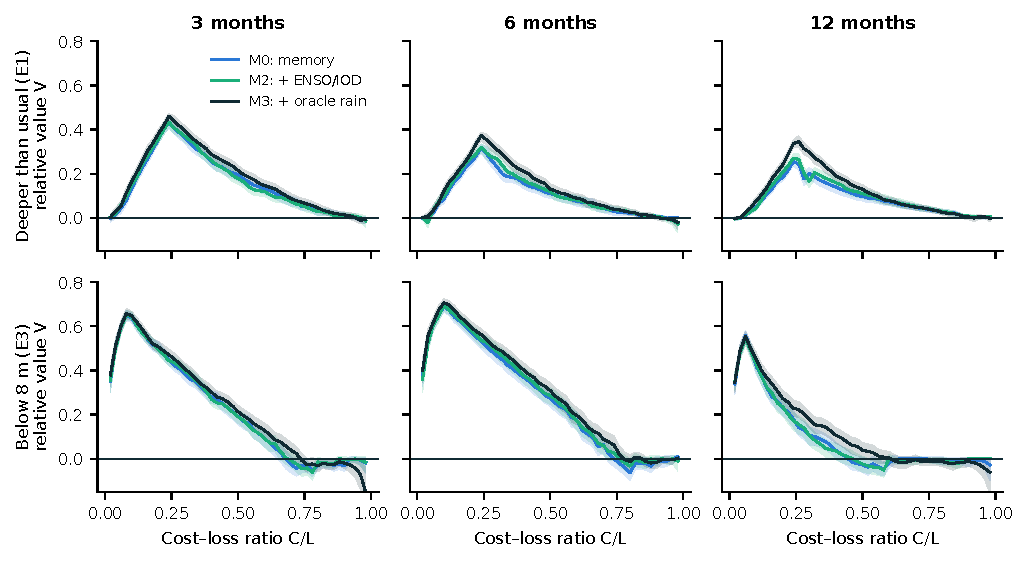
\includegraphics[width=\textwidth]{fig8}
\caption{Relative economic value of E1 and E3 warnings against the user's cost--loss ratio, for the memory-only, forcing and
oracle-rainfall models; bands are 95\,\% well-clustered intervals.}
\label{fig:value}
\end{figure*}

\section{Discussion}

\paragraph{Memory first, forcing second.} At national scale and seasonal lead times, the state of the aquifer explains most of
what can be forecast. Observed rainfall adds a few per cent, concentrated where hydrology says it should: shallow wells and the
monsoon-spanning forecast. That is consistent with Korean wells \citep{kim2026sources}, where past weather added little and
known future weather added most, and it reframes the value of climate information for Indian groundwater: the gain lies in
forecasting the coming monsoon, not in describing the last one.

\paragraph{Reproducing a null result.} The 2026 benchmark on the same file found that climate features added almost nothing. We
reproduce that result with the same construction and show that the feature is a single-day reading. Benchmarks built on public
compilations need a check of what each column measures.

\paragraph{Calibration under regime change.} Conformal guarantees assume that calibration and test residuals are exchangeable.
Monsoon variability breaks that assumption at the scale of years, and the break is visible in the residuals. Online
recalibration with adaptive conformal inference is cheap and restored conditional coverage without re-training; the same
mechanism applied to probabilities restored decision value. Interval coverage alone is not enough evidence for warning
probabilities.

\paragraph{Limitations.} Abstraction is not observed, so the models cannot separate a pumping response from a climate response
and cannot support pumping-quota optimisation. Most manual records in the compilation end in 2022--2023, so test campaigns after
2023 are thin. Regions are coarse latitude--longitude boxes, not aquifer polygons. The datum jumps were kept rather than cleaned.
Telemetry wells were not used for forecasting. The case study is at state level because an official district list of the Atal
Bhujal scheme was not available to us.

\section{Conclusions}

(1) Groundwater memory explains most seasonal forecast skill across India; observed monsoon forcing adds a small, robust gain,
largest at 6 months, and a perfect monsoon forecast would add \oracleMin--\oracleMax\,\% more. (2) The rainfall field of the
public compilation is a single-day snapshot and should not be used as forcing. (3) Conformal intervals pooled by depth and region
and updated online keep every depth and region class within about 3 points of nominal. (4) Warnings are worth acting on once their
probabilities are recalibrated on recent outcomes; the rule ``warn when $p \ge C/L$'' serves every user, with defaults of 0.3 for
seasonal planning and 0.2 for pump decisions six months ahead.

\section*{Code and data availability}
Code, processed results, figures and the dashboard are in the project repository (archive and DOI to be added on release). The
groundwater levels come from a public compilation of CGWB data; IMD gridded data were obtained with \texttt{imdlib}; Ni\~no~3.4
and DMI from NOAA PSL; state boundaries from geoBoundaries \citep{runfola2020geoboundaries}. Redistribution terms of the
groundwater compilation are being confirmed before processed data are archived.

\section*{Author contributions and competing interests}
To be completed by the author. The author declares no competing interests.

\bibliographystyle{abbrvnat}
\bibliography{../docs/references}

\end{document}
